\documentclass[12pt, french]{article}

\usepackage{fancyhdr, fancybox, lastpage}
\usepackage[most]{tcolorbox}
\usepackage[a4paper, margin={0.3in, .75in}]{geometry}
\usepackage{wrapfig}
\pagestyle{fancy}
\renewcommand\headrulewidth{1pt}
\renewcommand\footrulewidth{1pt}
\fancyhf{}
\rhead{ \em{Zakaria Haouzan}}
\lhead[C]{\em{2ème année baccalauréat Sciences Physiques}}
\chead[C]{}
\rfoot[C]{}
\lfoot[R]{}
\cfoot[]{\em{Page \thepage / \pageref{LastPage}}}


\newtcolorbox{Box2}[2][]{
                lower separated=false,
                colback=white,
colframe=white!20!black,fonttitle=\bfseries,
colbacktitle=white!30!gray,
coltitle=black,
enhanced,
attach boxed title to top left={yshift=-0.1in,xshift=0.15in},
title=#2,#1}


\begin{document}

\begin{center}

\vspace{-2cm}
   \shadowbox {\bf{ Modulation et démodulation d’amplitude}}
\end{center}

\vspace{-0.5cm}
%%_________________________Exercice ! :"_________________________Exercice
   \begin{Box2}{Exercice 1 : transmettre un signal $S(t)$ }
%  \begin{center}
	  %\vspace{-0.6cm}
	%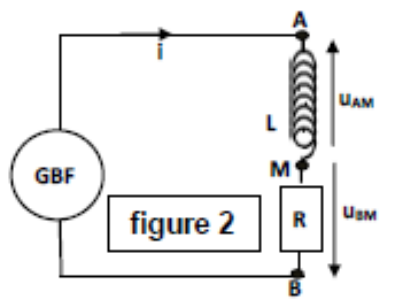
\includegraphics[width=0.22\textwidth]{./img/RL_ex00.png}
  %\end{center}
%\end{wrapfigure}

Pour transmettre un signal $S(t)$ de fréquence $f_S$, le groupe précédent
d’élèves, réalise dans un deuxième temps le montage de la figure 4, où ils ont
appliqué la tension $p(t) = P_mcos(2.\pi.F_P.t)$ sur l’entrée $E_1$ et la tension
$S(t) + U_0$=$S_mcos(2.\pi.f_S.t) + U_0$ sur l’entrée $E_2$. ($U_0$ la composante continue de la tension)

La visualisation des tensions $S(t) + U_0$ et $u_{S}(t)$ à la sortie du circuit
multiplieur, permet d’obtenir les courbes représentées sur les figures 5 et 6.
  \begin{center}
	  \vspace{-0.6cm}
	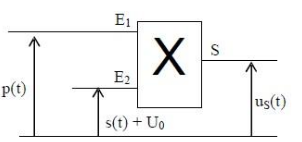
\includegraphics[width=0.32\textwidth]{./img/fig_ex00_1.png}
	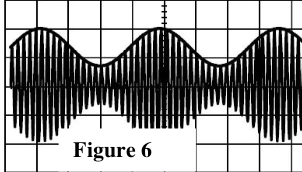
\includegraphics[width=0.32\textwidth]{./img/fig_ex00_2.png}
	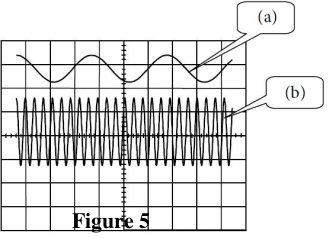
\includegraphics[width=0.32\textwidth]{./img/fig_ex00_3.png}
  \end{center}
\begin{enumerate}
	\item Quelle condition doit satisfaire
$F_P$ et $f_S$ pour obtenir une bonne
modulation ?
\item Affecter à chaque courbe des
figures 5 et 6, la tension
correspondante.

\item Déterminer le taux de modulation m, sachant que la sensibilité  verticale de l’oscilloscope est $1 V/div$. Conclure
\end{enumerate}


   \end{Box2}


%%_________________________Exercice !2 :"_________________________Exercice
\begin{Box2}{Exercice 2 : la modulation d’amplitude }
   % \begin{wrapfigure}[10]{r}{0.27\textwidth}
  %\begin{center}
	%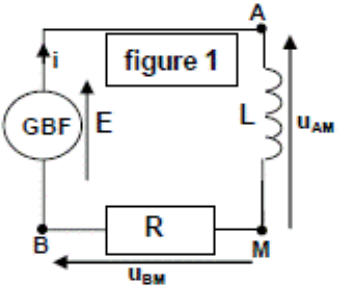
\includegraphics[width=0.22\textwidth]{./img/RL_ex01.png}
	%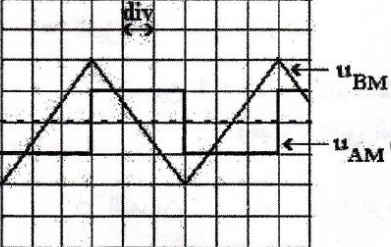
\includegraphics[width=0.27\textwidth]{./img/RL_ex01_1.png}
  %\end{center}
%\end{wrapfigure}

Pour étudier la modulation d’amplitude et vérifier la qualité de la modulation, au cours d’une séance de TP, le
professeur a utilisé avec ses élèves, un circuit intégré multiplieur (X)
en appliquant une tension sinusoïdale $u_1(t) = P_m.cos(2.\pi.F_p.t)$ à son
entrée $E_1$ et une tension $u_2(t) = U_0 + s(t)$ à son entrée $E_2$, avec $U_0$ la composante continue de la tension et $s(t)=S_m.cos(2.\pi.f_s.t)$ la tension modulante (figure 3).
  \begin{center}
	  \vspace{-0.6cm}
	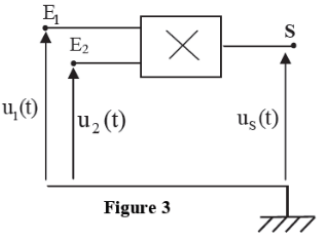
\includegraphics[width=0.32\textwidth]{./img/fig_ex01_1.png}
	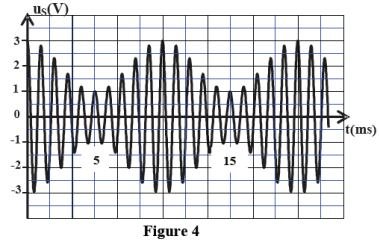
\includegraphics[width=0.42\textwidth]{./img/fig_ex01_2.png}
  \end{center}
La courbe de la figure 4 représente la tension de sortie
$u_s(t) = k.u_1(t).u_2(t)$, visualisée par les élèves sur l’écran d’un
oscilloscope. k est une constante positive caractérisant le multiplieur
X.

\begin{enumerate}
	\item Montrer, en précisant les expressions de A ,$u_S$(V) et de m, que
la tension $u_s(t)$ s’écrit sous la forme : $u_s(t) = A[1+m.cos(2.\pi.f_s.t)].cos(2.\pi.F_p.t)$ .

\item Trouver les fréquences $F_p$ de la porteuse et $f_s$ de la
tension modulante.

\item Déterminer le taux de modulation et en déduire la qualité
de modulation.

\end{enumerate}

\end{Box2}

%%_________________________Exercice ! 3:"_________________________Exercice
\begin{Box2}{Exercice 3 :Etablissement du courant dans le circuit primaire : }
%\begin{wrapfigure}{r}{0.12\textwidth}
  %\begin{center}
	%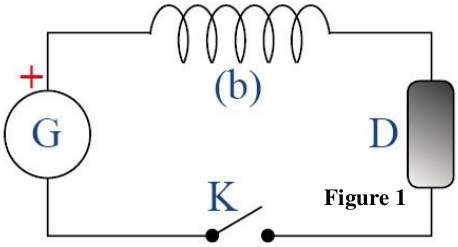
\includegraphics[width=0.12\textwidth]{./img/RL_ex02.png}
  %\end{center}
%\end{wrapfigure}
On utilise un résistor (D) de résistance $R= 100\Omega$ et un
condensateur (c) de capacité $C = 10\mu.F$, dans le détecteur de
crêtes correspondant à l’un des étages du circuit représenté
par la figure 3,
Pour détecter les crêtes de la tension modulée en
amplitude d’expression :
$$u(t) = k[0,5.cos(10^3.\pi.t) + 0,7].cos(10^4.\pi.t)$$
  \begin{center}
	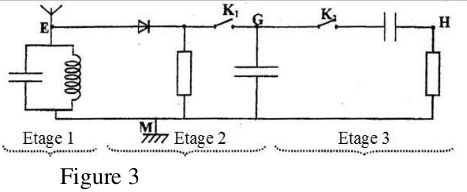
\includegraphics[width=0.42\textwidth]{./img/fig_ex02_1.png}
	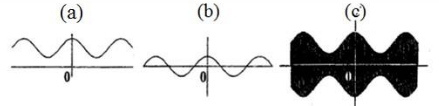
\includegraphics[width=0.42\textwidth]{./img/fig_ex02_2.png}
  \end{center}
\begin{enumerate}
\item  Indiquer, à l’aide de la figure 3, l’étage correspondant au détecteur de crêtes.
\item  Montrer que le dipôle $RC$ permet une bonne détection de crêtes.
\item  Les deux interrupteurs $K_1$ et $K_2$ sont fermés,
les courbes obtenus successivement sur l’écran
d’un oscilloscope
Représentent les variations des tensions uEM, uGM et uHM (Figure 4). Indiquer en justifiant, la courbe
\end{enumerate}

\end{Box2}

%%_________________________Exercice 4 : _________________________Exercice

%\vspace{2cm}
\begin{center}
\vspace{-0.7cm}
   \Large{ \em{Exercices Supplémentaires}}
\end{center}

\vspace{-0.7cm}

%%_________________________Exercice 5 : _________________________Exercice
\begin{Box2}{Exercice 4 :La  démodulation  d’amplitude }
   % \begin{wrapfigure}[15]{r}{0.27\textwidth}
  %\begin{center}
	  %%\vspace{-0.6cm}
	%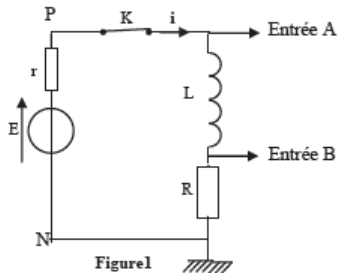
\includegraphics[width=0.2\textwidth]{./img/RLex031.png}
	%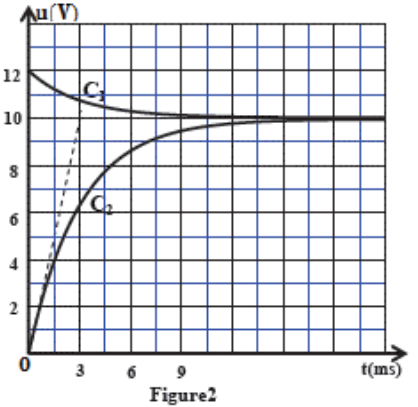
\includegraphics[width=0.27\textwidth]{./img/RL_ex32.png}
  %\end{center}
%\end{wrapfigure}

Pour transmettre un signal sinusoïdal s(t) on utilise un
multiplieur.

  \begin{center}
	  \vspace{-1cm} 
	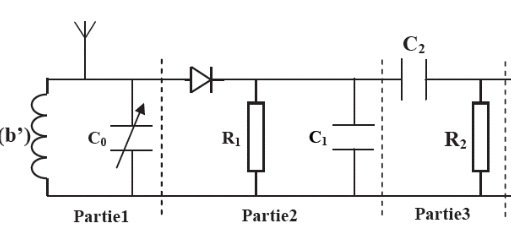
\includegraphics[width=0.44\textwidth]{./img/fig_ex03.png}
  \end{center}


On applique à l’entré $E_1$ du multiplieur un signal de tension
$u(t)=s(t)+V_0$ avec $V_0$ la tension continue de décalage, et on
applique à l’entrée $E_2$ p(t) une tension p(t) d’une onde porteuse . On obtient à la sortie S du multiplieur la tension
modulée en amplitude $u_S(t)$ telle que :
$$u_S(t) = A[1+0,6cos(10^4.\pi.t)].cos(2.10^5.\pi.t)$$
\begin{enumerate}
	\item  Montrer que la modulation d’amplitude
obtenue est bonne.
\item  La  démodulation  d’amplitude est réalisée à
l’aide du montage de la figure 6.
La partie 1 du montage comprend la bobine (b’) et un
condensateur de capacité $C_0$ réglable entre les deux
valeurs $6.10^{-12} F$ et $12.10^{-12} F$. Le conducteur ohmique
utilisé dans la partie 2 du montage a une résistance $R_1=30k\Omega$.
\begin{enumerate}
	
	\item  Montrer que l’utilisation de la bobine (b’) dans
le montage permet à la partie1 du montage de
sélectionner le signal uS(t).
\item  On veut obtenir une bonne détection d’enveloppe en utilisant l’un des condensateurs de capacités : $10 nF$ ;
5 nF ; 0,5 nF ; 0,1 nF . Déterminer la capacité du condensateur qui convient.
\end{enumerate}
\end{enumerate}
\end{Box2}
%%_________________________Exercice 6 : _________________________Exercice
%\begin{Box2}{Exercice 6 : échographie}
%%\begin{wrapfigure}{r}{0.2\textwidth}
  %%\begin{center}
	  %%\vspace{-0.6cm}
	%%\includegraphics[width=0.2\textwidth]{./img/Exercice6.png}
  %%\end{center}
%%\end{wrapfigure}


%\end{Box2}

\end{document}
